\documentclass[border=3pt,tikz]{standalone}
\usepackage{amsmath}
\usetikzlibrary{calc}
\usetikzlibrary{arrows.meta} % for arrow size
\begin{document}
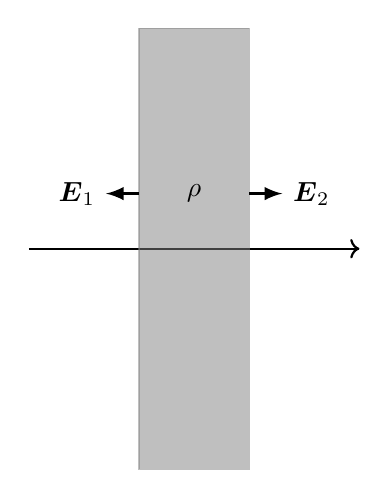
\begin{tikzpicture}[scale=1.4, rotate=0]
    \draw[thick, ->] (-1, 0) -- (2, 0); 
    
    % \draw[thick, ->] (0, 0) -- (0, 4) node [above] {$\hat{z}$};
    % \draw[thick, teal] (0,0) ellipse (2 and 0.5);
    % \node[above] at (1., -0.5) {$\lambda$};
    % \node[above] at(-1, 0) {$R$};
    % \draw[red, >-Stealth] (0, 0) -- (-2, 0);
    % \draw[black,fill=black] (0,2.5) circle (1pt) node [left] {$z$};
    \filldraw [gray,opacity=0.5] (0,-2) rectangle (1,2);
    \node at (0.5, 0.5) {$\rho$};
    \draw [very thick, -latex] (1, 0.5) -- (1.3, 0.5 ) node [right] {$\boldsymbol{E}_2$};
    \draw [very thick, -latex] (0.0, 0.5) -- (-0.3, 0.5 ) node [left] {$\boldsymbol{E}_1$};
  \end{tikzpicture}
\end{document}